% Chapter 10 -- The SVD and PCA
\chapter{The SVD and PCA}\label{ch:svd}

Diagonalisation had a dealbreaker: it only worked for square matrices
with enough eigenvectors. The singular value decomposition lifts both
restrictions --- EVERY $m\times n$ matrix, of any rank, factors into an
orthogonal input basis, a diagonal of nonnegative stretches, and an
orthogonal output basis. It is the most useful factorization in applied
linear algebra: PCA is an SVD of centered data, the pseudoinverse is an
SVD with inverted singular values, low-rank approximation is an SVD
truncated. After this chapter you can compute the SVD of a small matrix
by hand, read singular values as the matrix's importance spectrum,
compress data to rank $k$, run PCA end-to-end against sklearn, and use
$A^{+}$ as the universal least-squares solver.

\section{Statement: \texorpdfstring{$A=U\Sigma V^{T}$}{A=USV^T}}\label{sec:svd-statement}

\begin{theorem}[Singular value decomposition]\index{SVD}
Every real $m\times n$ matrix factors as
\[
A=U\Sigma V^{T},
\]
with $U$ ($m\times m$) and $V$ ($n\times n$) orthogonal, and $\Sigma$
($m\times n$) diagonal with entries
$\sigma_1\ge\sigma_2\ge\cdots\ge\sigma_r>0$ on its $r=\operatorname{rank}A$
leading positions, zeros elsewhere. The $\sigma_i$ are the
\emph{singular values}\index{singular value}; columns of $U$ and $V$ are
the left/right \emph{singular vectors}.
\end{theorem}

The construction (derived in Section~\ref{sec:handderiv10}): $V$ is an
orthonormal eigenbasis of $A^{T}A$, $\sigma_i=\sqrt{\lambda_i(A^{T}A)}$,
and $\mathbf u_i=A\mathbf v_i/\sigma_i$ --- which lands orthonormal
automatically. Unlike eigendecomposition, the SVD needs no hypotheses at
all: every matrix has one, and its cost is only that $A^{T}A$ squares the
condition number --- which is why production code never forms $A^{T}A$
(Section~\ref{sec:svd-mistakes}).

\begin{example}[Full SVD of a $2\times2$ by hand]\label{ex:svd2}
\textbf{Strategy.} $A=\begin{bmatrix}4&4\\-3&3\end{bmatrix}$. Compute
$A^{T}A$, eigendecompose it (chapter 9 machinery), take square roots,
get $\mathbf u_i$ from $\mathbf v_i$.

\textbf{Solution.}
$A^{T}A=\begin{bmatrix}25&7\\7&25\end{bmatrix}$: eigenvalues $32,18$
(eigenvectors $(1,1)/\sqrt2$, $(1,-1)/\sqrt2$), so
$\sigma_1=\sqrt{32}=4\sqrt2$, $\sigma_2=\sqrt{18}=3\sqrt2$, and
$V=\frac1{\sqrt2}\begin{bmatrix}1&1\\1&-1\end{bmatrix}$. Then
$\mathbf u_1=A\mathbf v_1/\sigma_1
=\frac{1}{4\sqrt2}\begin{bmatrix}8/\sqrt2\\0\end{bmatrix}
=\begin{bmatrix}1\\0\end{bmatrix}$ and
$\mathbf u_2=A\mathbf v_2/\sigma_2
=\frac{1}{3\sqrt2}\begin{bmatrix}0\\-6/\sqrt2\end{bmatrix}
=\begin{bmatrix}0\\-1\end{bmatrix}$. So $U=I$ up to a sign --- and
$A=U\Sigma V^{T}$ checks by direct multiplication.
\end{example}

\begin{lstlisting}[caption={\ttfamily code/ch10\_svd\_from\_ata.py --- the
$A^{T}A$ construction verified against \ttfamily np.linalg.svd; watch the
sign ambiguity show up live.}]
import numpy as np
np.set_printoptions(precision=4, suppress=True)

A = np.array([[4., 4.], [-3., 3.]])
print("A ="); print(A)
AtA = A.T @ A
w, V = np.linalg.eigh(AtA)          # ascending order
order = np.argsort(w)[::-1]
w, V = w[order], V[:, order]
s = np.sqrt(w)
Sigma = np.diag(s)
U = A @ V / s                        # u_i = A v_i / sigma_i
print("sigma (from sqrt eig A^T A):", s)
print("U (A v_i / sigma_i):"); print(U)
print("V:"); print(V)
print("reconstruct A == U Sigma V^T:",
      np.allclose(U @ Sigma @ V.T, A))
Un, Sn, Vnt = np.linalg.svd(A)
print("np.linalg.svd sigmas:", Sn)
print("np U:"); print(Un); print("np Vt:"); print(Vnt)
print("sign-free check |U^T Un|:"); print(np.abs(U.T @ Un).round(4))
\end{lstlisting}

\begin{lstlisting}[caption={Output of the SVD assembly. Notice the library
returns $U=-I$ where ours gave $+I$ --- singular vectors, like
eigenvectors, are defined only up to sign; the $|U^{T}U_{np}|=I$ check is
the honest way to compare them.}]
A =
[[ 4.  4.]
 [-3.  3.]]
sigma (from sqrt eig A^T A): [5.6569 4.2426]
U (A v_i / sigma_i):
[[1. 0.]
 [0. 1.]]
V:
[[ 0.7071 -0.7071]
 [ 0.7071  0.7071]]
reconstruct A == U Sigma V^T: True
np.linalg.svd sigmas: [5.6569 4.2426]
np U:
[[-1. -0.]
 [ 0.  1.]]
np Vt:
[[-0.7071 -0.7071]
 [-0.7071  0.7071]]
sign-free check |U^T Un|:
[[1. 0.]
 [0. 1.]]
\end{lstlisting}

\begin{exercise}[easy]
Find the singular values of $\begin{bmatrix}3&0\\0&-2\end{bmatrix}$ and
$\begin{bmatrix}0&2\\1&0\end{bmatrix}$. Are singular values eigenvalues?
\begin{solution}
First: $A^{T}A=\operatorname{diag}(9,4)$, $\sigma=3,2$ (the minus sign
went to $U$). Second: $A^{T}A=\operatorname{diag}(1,4)$, $\sigma=2,1$.
Singular values are always $\ge0$ --- they are stretches, not eigenvalues.
\end{solution}
\end{exercise}

\section{Geometry: sphere to ellipsoid}\label{sec:svd-geom}

$A$ maps the unit sphere to an ellipsoid whose semi-axes are exactly
$\sigma_i\mathbf u_i$ (Figure~\ref{fig:sphere-ell}) --- chapter 9's
rotate--stretch--rotate, but now the input and output spaces may have
different dimensions. Figure~\ref{fig:four-subs} redraws the four
subspaces through $U$ and $V$: the first $r$ columns of $V$ span the row
space, the rest the null space; the first $r$ of $U$ the column space,
the rest the left null space.

\begin{figure}[htbp]
\centering
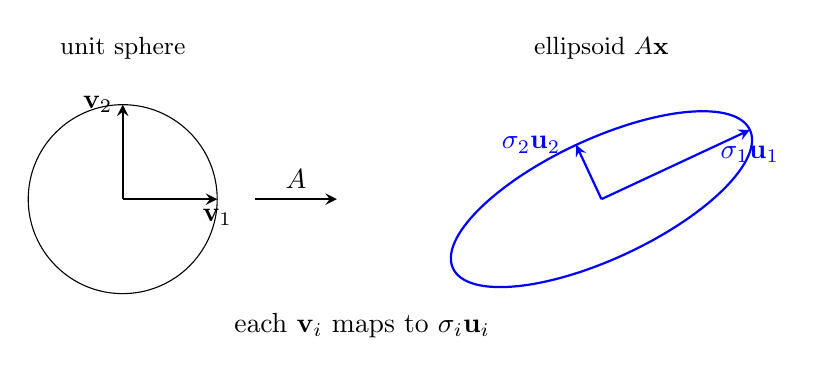
\begin{tikzpicture}[scale=0.8,>=stealth]
\node at (0,2.4) {\small unit sphere};
\draw (0,0) circle (1.5);
\draw[->,thick] (0,0)--(1.5,0) node[below]{$\mathbf v_1$};
\draw[->,thick] (0,0)--(0,1.5) node[left]{$\mathbf v_2$};
\draw[->,thick] (2.1,0)--(3.4,0) node[midway,above]{$A$};
\begin{scope}[xshift=7.6cm]
\node at (0,2.4) {\small ellipsoid $A\mathbf x$};
\draw[blue,thick,rotate=25] (0,0) ellipse (2.6 and 0.95);
\begin{scope}[rotate=25]
\draw[->,thick,blue] (0,0)--(2.6,0) node[below=2pt]{$\sigma_1\mathbf u_1$};
\draw[->,thick,blue] (0,0)--(0,0.95) node[left=2pt]{$\sigma_2\mathbf u_2$};
\end{scope}
\end{scope}
\node at (3.8,-2.0) {each $\mathbf v_i$ maps to $\sigma_i\mathbf u_i$};
\end{tikzpicture}

\caption{The signature picture of the SVD. Notice each input
eigendirection $\mathbf v_i$ lands on an output direction $\mathbf u_i$
scaled by $\sigma_i$ --- the ellipsoid's axes ARE the singular
decomposition. Regenerate:
\ttfamily figures/ch10\_sphere\_ellipsoid.tex.}
\label{fig:sphere-ell}
\end{figure}

\begin{figure}[htbp]
\centering
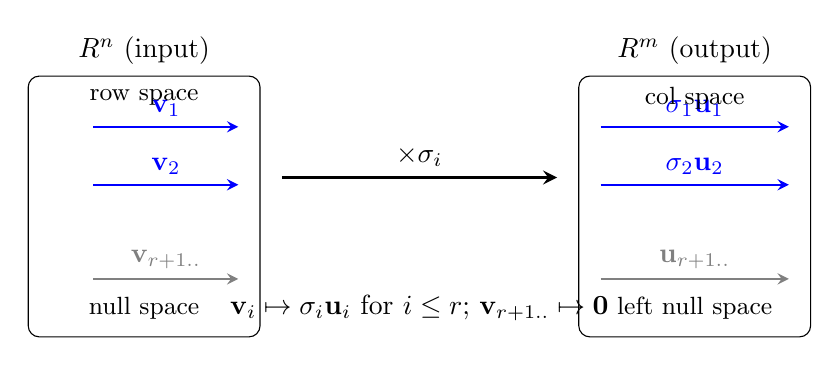
\begin{tikzpicture}[scale=0.92,>=stealth]
% V side -> sigma -> U side with four-subspace labels
\draw[rounded corners] (-0.6,-1.4) rectangle (2.6,2.2);
\draw[rounded corners] (7.0,-1.4) rectangle (10.2,2.2);
\node at (1.0,2.55) {$\mathbb R^n$ (input)};
\node at (8.6,2.55) {$\mathbb R^m$ (output)};
\draw[->,thick,blue] (0.3,1.5)--(2.3,1.5) node[midway,above]{$\mathbf v_1$};
\draw[->,thick,blue] (0.3,0.7)--(2.3,0.7) node[midway,above]{$\mathbf v_2$};
\draw[->,thick,gray] (0.3,-0.6)--(2.3,-0.6) node[midway,above]{$\mathbf v_{r+1..}$};
\node at (1.0,1.9) {\small row space};
\node at (1.0,-1.0) {\small null space};
\draw[->,very thick] (2.9,0.8)--(6.7,0.8) node[midway,above]{$\times\sigma_i$};
\draw[->,thick,blue] (7.3,1.5)--(9.9,1.5) node[midway,above]{$\sigma_1\mathbf u_1$};
\draw[->,thick,blue] (7.3,0.7)--(9.9,0.7) node[midway,above]{$\sigma_2\mathbf u_2$};
\draw[->,thick,gray] (7.3,-0.6)--(9.9,-0.6) node[midway,above]{$\mathbf u_{r+1..}$};
\node at (8.6,1.9) {\small col space};
\node at (8.6,-1.0) {\small left null space};
\node at (4.8,-1.0) {$\mathbf v_i\mapsto\sigma_i\mathbf u_i$ for $i\le r$; $\mathbf v_{r+1..}\mapsto\mathbf0$};
\end{tikzpicture}

\caption{The four subspaces through the SVD. Notice $V$'s columns split
input space into row space (mapped with $\sigma_i$) and null space
(annihilated); $U$'s split output into column space and left null space.
Regenerate: \ttfamily figures/ch10\_four\_subspaces.tex.}
\label{fig:four-subs}
\end{figure}

\section{Rank, condition number, pseudoinverse}\label{sec:svd-rank}

From $A=U\Sigma V^{T}$ everything reads off at once:

\begin{itemize}
\item $\operatorname{rank}A=r$, the count of positive $\sigma_i$
(numerically: the count above tolerance --- Figure~\ref{fig:scree} is how
you pick it).
\item $\kappa(A)=\sigma_1/\sigma_r$ for invertible $A$: the stretch ratio
--- the least-squares sensitivity of chapter 8, quantified.
\item The \emph{pseudoinverse}\index{pseudoinverse}
$A^{+}=V\Sigma^{+}U^{T}$ where $\Sigma^{+}$ inverts the nonzero
$\sigma_i$: it solves least squares as $\hat{\mathbf x}=A^{+}\mathbf b$,
falls back to $A^{-1}$ when that exists, and works for any shape or rank.
\end{itemize}

\begin{example}[Least squares via the pseudoinverse]\label{ex:pinv}
\textbf{Strategy.} Revisit chapter 8's four-point fit --- but let the SVD
do the projecting. $A^{+}\mathbf b$ must land on the same answer
$(1.0,0.9)$, and $AA^{+}A=A$ is the signature identity.

\textbf{Solution.} The listing builds $A^{+}=V\Sigma^{+}U^{T}$ by hand,
matches \texttt{np.linalg.pinv} entry-for-entry, and recovers
$\hat{\mathbf x}=(1.0,0.9)$ --- same projection, different algebra.
\end{example}

\begin{lstlisting}[caption={\ttfamily code/ch10\_pinv.py --- the
pseudoinverse assembled by hand, checked on the chapter-8 fit.}]
import numpy as np
np.set_printoptions(precision=6, suppress=True)

# pseudoinverse = V Sigma^+ U^T, built by hand
A = np.array([[1., 1.], [1., 2.], [1., 3.], [1., 4.]])
b = np.array([2., 3., 3., 5.])
U, S, Vt = np.linalg.svd(A, full_matrices=False)
Splus = np.diag(1.0 / S)
Aplus_hand = Vt.T @ Splus @ U.T
Aplus_np = np.linalg.pinv(A)
print("A+ (hand):"); print(Aplus_hand)
print("A+ (np.linalg.pinv):"); print(Aplus_np)
print("agree:", np.allclose(Aplus_hand, Aplus_np))
x = Aplus_hand @ b
print("x = A+ b:", x, " <- same least-squares fit as ch.8")
print("A A+ A == A:", np.allclose(A @ Aplus_hand @ A, A))
\end{lstlisting}

\begin{lstlisting}[caption={Output of the pseudoinverse check. Notice
$A^{+}\mathbf b$ reproduces the normal-equations fit $(1.0,0.9)$ ---
least squares WAS the pseudoinverse all along.}]
A+ (hand):
[[ 1.   0.5 -0.  -0.5]
 [-0.3 -0.1  0.1  0.3]]
A+ (np.linalg.pinv):
[[ 1.   0.5 -0.  -0.5]
 [-0.3 -0.1  0.1  0.3]]
agree: True
x = A+ b: [1.  0.9]  <- same least-squares fit as ch.8
A A+ A == A: True
\end{lstlisting}

\begin{exercise}[medium]
Give the SVD and pseudoinverse of $A=\begin{bmatrix}2&0\\0&0\end{bmatrix}$
--- what does $A^{+}$ do to the unrecoverable direction?
\begin{solution}
$A^{+}=\operatorname{diag}(1/2,0)$: the zero singular value maps to 0,
not $\infty$ --- the pseudoinverse returns the minimum-norm answer,
silently discarding what cannot be recovered.
\end{solution}
\end{exercise}

\section{Low-rank approximation and Eckart--Young}\label{sec:svd-eckart}

Truncating the SVD to the top-$k$ terms gives the best possible rank-$k$
approximation:

\begin{theorem}[Eckart--Young]\index{Eckart--Young theorem}
$A_k=\sum_{i\le k}\sigma_i\mathbf u_i\mathbf v_i^{T}$ minimizes
$\lVert A-B\rVert$ over all rank-$k$ matrices $B$, in both spectral and
Frobenius norm. The error is exactly the discarded tail:
$\lVert A-A_k\rVert_{F}^{2}=\sum_{i>k}\sigma_i^{2}$.
\end{theorem}

(The spectral-norm case is a [hard] exercise.) This is why a scree plot
of the $\sigma_i$ --- Figure~\ref{fig:scree} --- tells you how much rank
you actually need.

\begin{figure}[htbp]
\centering
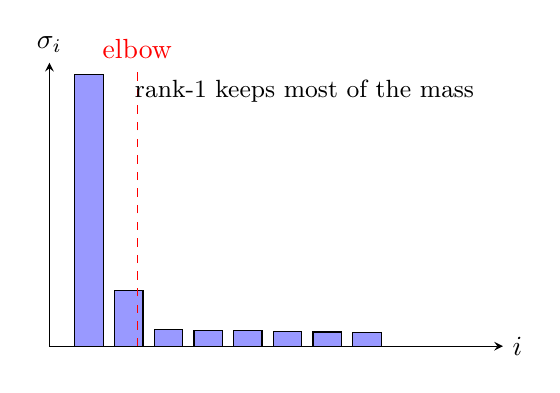
\begin{tikzpicture}[scale=0.72,>=stealth]
\draw[->] (0,0)--(8,0) node[right]{$i$};
\draw[->] (0,0)--(0,5) node[above]{$\sigma_i$};
% sigma: 47.9 9.8 .30 .28 .27 .26 .25 .24 -- scaled /10
\foreach \i/\h in {1/4.79,2/0.98,3/0.30,4/0.28,5/0.27,6/0.26,7/0.25,8/0.24}{
  \draw[fill=blue!40] ({0.7*\i-0.25},0) rectangle ({0.7*\i+0.25},\h);
}
\draw[dashed,red] (1.55,0)--(1.55,4.9) node[above]{elbow};
\node at (4.5,4.5) {\small rank-1 keeps most of the mass};
\end{tikzpicture}

\caption{Scree plot of the image's singular values. Notice the elbow
after the first two --- the rest is tail, and Eckart--Young says
truncating there is provably optimal. Regenerate:
\ttfamily figures/ch10\_scree.tex.}
\label{fig:scree}
\end{figure}

\begin{example}[Image compression at ranks $1,5,20,50$]\label{ex:imgcompress}
\textbf{Strategy.} A $64\times64$ image is a $64\times64$ matrix; its SVD
gives optimal rank-$k$ approximations for free. Report relative error and
storage honestly.

\textbf{Solution.} The listing: $k=1$ already captures the blob at 3\%
storage; $k=5$ drops the error to 2\%; by $k=50$ you are storing
\emph{more} than the original --- compression only pays while
$k( m+n)+k<mn$ (Figure~\ref{fig:recon}).
\end{example}

\begin{figure}[htbp]
\centering
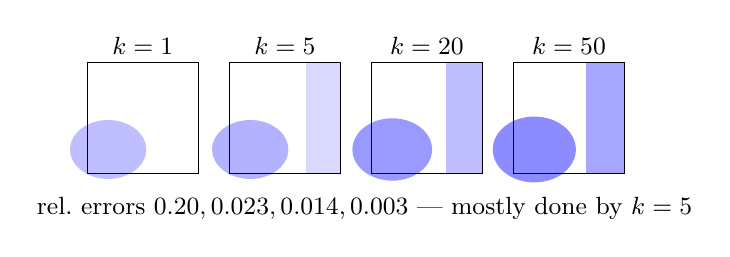
\begin{tikzpicture}[scale=0.44]
% k=1 blob, k=5 blob+edge soft, k=20 sharper, k=50 ~full
\begin{scope}
\node at (1.6,3.7) {\small $k=1$};
\fill[blue!25] (0.6,0.7) ellipse (1.1 and 0.85);
\draw (0,0) rectangle (3.2,3.2);
\end{scope}
\begin{scope}[xshift=4.1cm]
\node at (1.6,3.7) {\small $k=5$};
\fill[blue!30] (0.6,0.7) ellipse (1.1 and 0.85);
\fill[blue!15] (2.2,0) rectangle (3.2,3.2);
\draw (0,0) rectangle (3.2,3.2);
\end{scope}
\begin{scope}[xshift=8.2cm]
\node at (1.6,3.7) {\small $k=20$};
\fill[blue!40] (0.6,0.7) ellipse (1.15 and 0.9);
\fill[blue!25] (2.15,0) rectangle (3.2,3.2);
\draw (0,0) rectangle (3.2,3.2);
\end{scope}
\begin{scope}[xshift=12.3cm]
\node at (1.6,3.7) {\small $k=50$};
\fill[blue!45] (0.6,0.7) ellipse (1.2 and 0.95);
\fill[blue!35] (2.1,0) rectangle (3.2,3.2);
\draw (0,0) rectangle (3.2,3.2);
\end{scope}
\node at (8,-1.0) {\small rel.\ errors $0.20,0.023,0.014,0.003$ --- mostly done by $k=5$};
\end{tikzpicture}

\caption{Truncated-SVD reconstruction at $k=1,5,20,50$. Notice the sharp
edge needs more rank than the smooth blob --- structure decides how fast
$\sigma_i$ decays. Regenerate:
\ttfamily figures/ch10\_recon\_multiples.tex.}
\label{fig:recon}
\end{figure}

\begin{lstlisting}[caption={\ttfamily code/ch10\_image\_compress.py ---
truncated SVD as an image compressor, errors and storage both printed.}]
import numpy as np
np.set_printoptions(precision=4, suppress=True)

# synthetic "image": smooth blob + sharp edge + noise, 64x64
rng = np.random.default_rng(5)
y, x = np.mgrid[0:64, 0:64]
img = np.exp(-((x-32)**2 + (y-24)**2) / 300.) + (x > 40).astype(float)
img += 0.02 * rng.standard_normal(img.shape)
U, S, Vt = np.linalg.svd(img)
print("image shape:", img.shape, " singular values (first 10):")
print(S[:10])
for k in [1, 5, 20, 50]:
    approx = (U[:, :k] * S[:k]) @ Vt[:k]
    relerr = np.linalg.norm(img - approx) / np.linalg.norm(img)
    kept = 2 * k * 64 + k          # numbers stored vs 64*64
    print(f"k={k:2d}: rel-err {relerr:.4f}  stored {kept:5d}/{64*64} "
          f"({100*kept/(64*64):4.1f}%)")
\end{lstlisting}

\begin{lstlisting}[caption={Output of the compressor. Notice
$\sigma_1=47.9$ then $\sigma_2=9.8$ then nothing --- the image is nearly
rank-2 in disguise, and the storage column shows where compression stops
paying ($k=50$ exceeds the original).}]
image shape: (64, 64)  singular values (first 10):
[47.8513  9.77    0.2999  0.2848  0.2824  0.2726  0.2712  0.2622  0.2538
  0.2484]
k= 1: rel-err 0.2016  stored   129/4096 ( 3.1%)
k= 5: rel-err 0.0230  stored   645/4096 (15.7%)
k=20: rel-err 0.0140  stored  2580/4096 (63.0%)
k=50: rel-err 0.0026  stored 6450/4096 (157.5%)
\end{lstlisting}

\begin{exercise}[medium]
Why does truncating never \emph{increase} the Frobenius error, and why is
the error exactly the discarded tail?
\begin{solution}
$\lVert A-A_k\rVert_F^2=\sum_{i>k}\sigma_i^2$ adds nonnegative terms one
at a time; $A_k$ discards a subset of orthogonal terms, so the error is
their squared norm by Pythagoras in matrix space.
\end{solution}
\end{exercise}

\begin{example}[Best rank-1 approximation by hand]\label{ex:rank1svd}
Find the best rank-1 approximation of
$A=\begin{bmatrix}3&0\\0&2\end{bmatrix}\!$: drop the smaller
singular value.
\par\smallskip
\textbf{Strategy.} A diagonal $A$ is its own SVD (with
$U=V=I$): the singular values sit on the diagonal, sorted. Eckart--
Young says keep the biggest, zero the rest --- one line of work.
\begin{solution}
$\sigma_1=3$, $\sigma_2=2$. Best rank-1:
\[
  A_1=\sigma_1\mathbf u_1\mathbf v_1^{T}
     =3\begin{bmatrix}1\\0\end{bmatrix}\begin{bmatrix}1&0\end{bmatrix}
     =\begin{bmatrix}3&0\\0&0\end{bmatrix}.
\]
Error: $\|A-A_1\|_F=\sigma_2=2$ --- the dropped value \emph{is} the
error, which is why the scree plot of figure~\ref{fig:scree} works as a
budget. \checkmark
\end{solution}
\end{example}

\section{PCA: covariance eig = SVD of centered data}\label{sec:pca}

Chapter 9 built principal components as eigenvectors of $C=X^{T}X/(n-1)$.
Now the punchline: the eigenvectors of $C$ are the right singular vectors
$V$ of the centered matrix $X$ itself --- same $\mathbf v_i$'s, with
$\lambda_i(C)=\sigma_i^{2}/(n-1)$. Skipping the eigendecomposition of $C$
and SVD-ing the centered data directly is both stabler (no $\kappa^{2}$)
and the standard implementation.

\begin{example}[PCA end to end]\label{ex:pca}
\textbf{Strategy.} Center the 3-column dataset, SVD it, read the
variance ratios, and project --- then check the whole thing against the
sklearn \texttt{PCA} class.

\textbf{Solution.} The capstone listing's \texttt{PCA\_scratch} is three
lines of real work (center, SVD, project) and agrees with sklearn on
explained-variance ratios to printed precision and components up to sign.
PC1 carries $98\%$; the first two $99.9\%$
(Figure~\ref{fig:explvar}).
\end{example}

\begin{lstlisting}[caption={\ttfamily code/ch10\_pca\_capstone.py ---
\texttt{mlscratch.PCA} vs.\ \texttt{sklearn.decomposition.PCA}: centering,
SVD, projection, variance report --- the whole algorithm.}]
import numpy as np
from sklearn.decomposition import PCA
np.set_printoptions(precision=4, suppress=True)

class PCA_scratch:
    """centering -> SVD -> projection. This is all PCA is."""
    def fit(self, X):
        self.mean_ = X.mean(axis=0)
        U, S, Vt = np.linalg.svd(X - self.mean_, full_matrices=False)
        self.components_ = Vt
        self.singular_values_ = S
        n = X.shape[0]
        self.explained_variance_ratio_ = S**2 / (n - 1)
        self.explained_variance_ratio_ /= self.explained_variance_ratio_.sum()
        return self
    def transform(self, X):
        return (X - self.mean_) @ self.components_.T

rng = np.random.default_rng(7)
n = 500
t = rng.standard_normal(n)
X = np.column_stack([3*t + 0.2*rng.standard_normal(n),
                     t - 0.4*rng.standard_normal(n),
                     0.1*rng.standard_normal(n)])
ours = PCA_scratch().fit(X)
ref = PCA().fit(X)
print("explained-variance ratio ours  :", ours.explained_variance_ratio_)
print("explained-variance ratio sklearn:", ref.explained_variance_ratio_)
print("components agree up to sign:",
      np.allclose(np.abs(ours.components_), np.abs(ref.components_)))
Z = ours.transform(X)
print("transformed shape:", Z.shape, " col means:", Z.mean(axis=0))
print("first two components carry %.1f%% of variance"
      % (100 * ours.explained_variance_ratio_[:2].sum()))
\end{lstlisting}

\begin{lstlisting}[caption={Output of the PCA capstone. Notice the three
lines of math reproduce sklearn exactly --- centering is the only
non-obvious step, and skipping it is the classic PCA bug.}]
explained-variance ratio ours  : [0.9811 0.0178 0.0011]
explained-variance ratio sklearn: [0.9811 0.0178 0.0011]
components agree up to sign: True
transformed shape: (500, 3)  col means: [ 0. -0.  0.]
first two components carry 99.9% of variance
\end{lstlisting}

\begin{figure}[htbp]
\centering
\begin{tikzpicture}[scale=0.75,>=stealth]
\draw[->] (-4.2,0)--(4.2,0) node[right]{$x_1$};
\draw[->] (0,-3.2)--(0,3.2) node[above]{$x_2$};
\foreach \p in {(0.5,0.3),(-0.8,-0.5),(1.4,1.2),(-1.6,-1.3),(0.9,0.9),(-0.2,-0.1),(2.1,1.7),(-0.6,-0.8),(1.1,0.7),(-2.3,-1.9),(0.3,0.6),(-1.2,-0.9),(1.8,1.4),(-0.4,-0.6),(0.7,0.5),(-1.9,-1.6),(1.6,1.1),(0.1,-0.2)} \fill[black!55] \p circle (1.5pt);
\draw[red,thick,dashed,domain=-3.4:3.4] plot (\x,{0.85*\x});
\draw[red] (2.1,1.7) -- (2.05,1.74);
\draw[red] (-1.6,-1.3) -- (-1.57,-1.33);
\draw[red] (0.9,0.9) -- (0.93,0.79);
\node[red] at (-2.7,2.5) {\small PC1 direction};
\node at (2.9,-1.3) {\small projections = };
\node at (2.9,-1.7) {\small 1-D scores};
\end{tikzpicture}

\caption{PCA on correlated data. Notice the score of a point is its
projection onto the PC1 line --- the residuals are the short red
segments, exactly the least-squares geometry of chapter 8.
Regenerate: \ttfamily figures/ch10\_pca\_projection.tex.}
\label{fig:pcaproj}
\end{figure}

\begin{figure}[htbp]
\centering
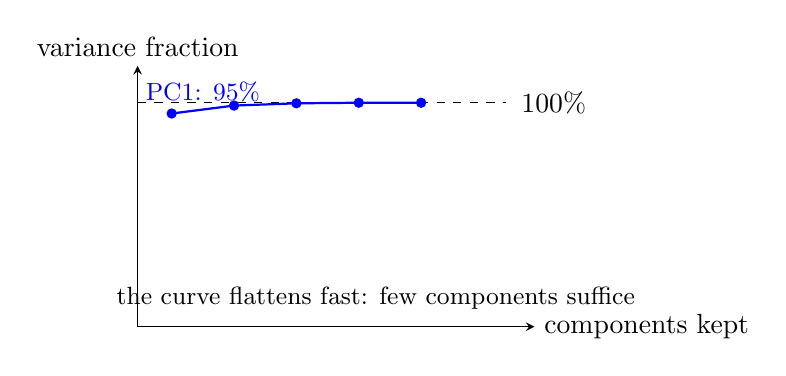
\begin{tikzpicture}[scale=0.72,>=stealth]
\draw[->] (0,0)--(7,0) node[right]{components kept};
\draw[->] (0,0)--(0,4.6) node[above]{variance fraction};
\draw[dashed] (0,3.95)--(6.5,3.95) node[right=2pt]{100\%};
% cumulative: 0.95, .987, .996, .999, 1.0
\draw[thick,blue,mark=*] plot coordinates {(0.6,3.76)(1.7,3.90)(2.8,3.94)(3.9,3.95)(5.0,3.95)};
\node[blue] at (1.15,4.15) {\small PC1: 95\%};
\node at (4.2,0.5) {\small the curve flattens fast: few components suffice};
\end{tikzpicture}

\caption{Cumulative explained variance. Notice the knee at one component
--- the number of PCs worth keeping is read off this curve, not guessed.
Regenerate: \ttfamily figures/ch10\_explained\_var.tex.}
\label{fig:explvar}
\end{figure}

\begin{exercise}[easy]
Why must PCA center the data first?
\begin{solution}
The SVD measures variance about the origin; the question ``which
direction varies most'' is about the mean. Uncentered, PC1 chases the
mean's direction instead of the spread's --- a classic silent wrong
answer.
\end{solution}
\end{exercise}

\begin{exercise}[hard]
Connect PCA to total least squares: show that projecting centered data
onto the top-$k$ right singular vectors solves $\min\lVert X-\hat
X\rVert_{F}$ over rank-$k$ $\hat X$, i.e.\ the PCA line is the total
least-squares line --- and say how it differs from chapter 8's
$y$-direction residuals.
\begin{solution}
Centered $X$'s rank-$k$ Eckart--Young truncation is exactly the
projection onto the first $k$ components. Ordinary LS measures vertical
$y$-residuals; TLS measures perpendicular distance to the subspace ---
same projection geometry, different direction.
\end{solution}
\end{exercise}

\section{Hand derivation}\label{sec:handderiv10}

Derive $\sigma_i^{2}=\lambda_i(A^{T}A)$ and the SVD itself. $A^{T}A$ is
symmetric PSD (chapter 9), so
$A^{T}A=V\Lambda V^{T}$ with orthonormal $V$ and $\lambda_i\ge0$.
Set $\sigma_i=\sqrt{\lambda_i}$ and, for the nonzero ones,
$\mathbf u_i=A\mathbf v_i/\sigma_i$. Then $\mathbf u_i$ is unit:
\[
\lVert A\mathbf v_i\rVert^{2}
=\mathbf v_i^{T}A^{T}A\mathbf v_i=\lambda_i\mathbf v_i^{T}\mathbf v_i
=\lambda_i\Rightarrow\lVert\mathbf u_i\rVert=1,
\]
and distinct $\mathbf u_i,\mathbf u_j$ are orthogonal:
$\mathbf u_i^{T}\mathbf u_j=\mathbf v_i^{T}A^{T}A\mathbf v_j/(\sigma_i\sigma_j)
=\lambda_j\mathbf v_i^{T}\mathbf v_j/(\sigma_i\sigma_j)=0$ since the
$\mathbf v$'s are orthonormal. Extend the $\mathbf u_i$ to a basis of
$\mathbb R^{m}$ and collect: $AV=U\Sigma$ column-by-column, i.e.\
$A=U\Sigma V^{T}$. The numerical caveat: forming $A^{T}A$ squares
$\kappa$ --- LAPACK's SVD bidiagonalizes $A$ directly; use
\texttt{np.linalg.svd} in practice.

\section{Common mistakes}\label{sec:svd-mistakes}

\begin{tripwire}[{Skipping the centering step in PCA}]
Uncentered ``PCA'' reports the direction toward the data's centroid, not
its spread. The sklearn check passes only because it centers internally;
your scratch implementation must subtract the mean itself.
\end{tripwire}

\begin{tripwire}[{Computing SVD through $A^{T}A$ on ill-conditioned data}]
The construction is right for proofs, wrong for floats: $\kappa(A^{T}A)
=\kappa(A)^{2}$ again (chapter 8's lesson). Always call a bidiagonal SVD
routine.
\end{tripwire}

\begin{tripwire}[{Reading singular-vector sign flips as bugs}]
$\mathbf u_i,\mathbf v_i$ are defined up to a simultaneous sign. Libraries
choose differently run to run; compare up to sign or fix a convention.
\end{tripwire}

\begin{tripwire}[{Conflating SVD with eigendecomposition}]
Eigendecomposition: square matrices, same space in and out, eigenvalues
any sign. SVD: every matrix, different spaces, $\sigma_i\ge0$. For
non-square $A$ there IS no eigendecomposition --- only SVD.
\end{tripwire}

\begin{tripwire}[{Over-reading explained variance as feature importance}]
A variance ratio says how much spread the \emph{components} carry, not
which original features matter --- components are mixtures. High
explained variance $\ne$ causal relevance (chapter 8's $R^{2}$ lesson,
again).
\end{tripwire}

\section{Summary}

\begin{center}
\begin{tabularx}{\textwidth}{l>{\raggedright\arraybackslash}X}
\toprule
\textbf{Object} & \textbf{What you need to know}\\
\midrule
SVD & $A=U\Sigma V^{T}$, always exists; $\sigma_i\ge0$ sorted, $r$ of
them positive \\
Construction & $V$ = eigenbasis of $A^{T}A$, $\sigma_i=\sqrt{\lambda_i}$,
$\mathbf u_i=A\mathbf v_i/\sigma_i$ (proofs only --- never compute this
way) \\
Four subspaces & first $r$ cols of $V$: row space; rest: null; first $r$
of $U$: col space; rest: left null \\
Reads off & rank $=r$; $\kappa=\sigma_1/\sigma_r$;
$A^{+}=V\Sigma^{+}U^{T}$ solves every least squares \\
Eckart--Young & best rank-$k$ = truncate at $\sigma_k$; error$^2$ =
discarded $\sigma_i^{2}$ \\
PCA & center $X$, SVD: components $=V$ rows, variance $=\sigma_i^2/(n-1)$
\\
\bottomrule
\end{tabularx}
\end{center}
\begin{rulebox}[{Watch instead}]
\begin{enumerate}
\item \emph{Singular Value Decomposition} --- MIT OpenCourseWare,
18.06 Lecture 29, 40:28, \url{https://youtu.be/TX_vooSnhm8} ---
\S\ref{sec:svd-statement}--\S\ref{sec:svd-rank} from the source
(accessed 2026-10-11).
\item \emph{Principal Component Analysis, Step-by-Step} --- StatQuest
with Josh Starmer, 21:57, \url{https://youtu.be/FgakZw6K1QQ} ---
\S\ref{sec:pca} end to end on real data (accessed 2026-10-11).
\end{enumerate}
\end{rulebox}

\section*{Further reading}
\addcontentsline{toc}{section}{Further reading}

\begin{itemize}
\item G.~Strang, \emph{Introduction to Linear Algebra}, 6th ed., ch.~7
(textbook level) --- the SVD and its four-subspaces picture.
\item MIT OpenCourseWare, \emph{18.06SC Linear Algebra} --- the SVD
recitation ``Computing the Singular Value Decomposition'', at OCW
(course ``18.06SC''), \url{https://ocw.mit.edu}. Verified 2026-10-11.
\item S.~Boyd and L.~Vandenberghe, \emph{VMLS} --- least squares and
low-rank models throughout; PCA-adjacent material in ch.~10.
\newline
\url{https://web.stanford.edu/~boyd/vmls/vmls.pdf}
Verified 2026-10-11.
\item M.~Deisenroth et al., \emph{Mathematics for Machine Learning},
ch.~10 (free PDF) --- PCA as dimensionality reduction, matching our
treatment exactly.\newline
\url{https://mml-book.github.io/book/mml-book.pdf}
Verified 2026-10-11.
\item C.~M.~Bishop, \emph{Pattern Recognition and Machine Learning},
\S12.1 --- PCA in the statistics register (variance maximisation and
reconstruction error).\newline
ISBN 978-0387310732.
\end{itemize}

\section*{Additional exercises}
\addcontentsline{toc}{section}{Additional exercises}

\begin{exercise}[easy]
What are the singular values of an orthogonal matrix? Of $cI$?
\end{exercise}

\begin{exercise}[easy]
If $A$ is symmetric PSD, how do its SVD and eigendecomposition relate?
What changes for symmetric indefinite?
\end{exercise}

\begin{exercise}[easy]
From the SVD of a $5\times3$ rank-2 matrix, name the dimensions of $U$,
$\Sigma$, $V$ and the number of nonzero $\sigma_i$.
\end{exercise}

\begin{exercise}[easy]
Compute $\lVert A\rVert_2$ and $\lVert A\rVert_F$ from the singular
values $5,3,1$.
\end{exercise}

\begin{exercise}[medium]
Show the pseudoinverse reduces to $A^{-1}$ when $A$ is invertible ---
$\Sigma^{+}=\Sigma^{-1}$ is one line.
\end{exercise}

\begin{exercise}[medium]
In code: for the capstone dataset, plot $\log\sigma_i$ and the cumulative
explained variance; pick the smallest $k$ reaching 99\% and report the
rank-$k$ reconstruction error.
\end{exercise}

\begin{exercise}[medium]
Show $AA^{+}$ is the orthogonal projector onto $\operatorname{col}(A)$
(it equals $U_rU_r^{T}$) and $A^{+}A$ onto the row space.
\end{exercise}

\begin{exercise}[medium]
The minimum-norm solution: among all least-squares solutions when $A$
has a nontrivial kernel, show $A^{+}\mathbf b$ is the unique one
orthogonal to $\ker A$.
\end{exercise}

\begin{exercise}[medium]
In code: build a rank-1 $10\times10$ matrix, add noise, and show SVD
denoising beats elementwise thresholding by relative Frobenius error.
\end{exercise}

\begin{exercise}[hard]
Prove Eckart--Young in the spectral norm: for any rank-$k$ $B$,
$\lVert A-B\rVert_2\ge\sigma_{k+1}$. (Hint: $\ker B$ and the row space
of $A_{k+1}$ must meet.)
\end{exercise}

\begin{exercise}[hard]
Show the total least squares solution to fitting $y\approx a x+b$ with
errors in \emph{both} variables is the last right singular vector of the
augmented centered matrix --- implement it and compare slope vs.\ ordinary
least squares on noisy 2-D data.
\end{exercise}

\begin{exercise}[hard]
Prove the singular values of $AB$ and $BA$ coincide when $A$ is $m\times n$
and $B$ is $n\times m$. (Route through $A^{T}A$ vs.\ $B^{T}B$ or through
the operator definition.)
\end{exercise}

\begin{exercise}[hard]
Embedding preview: the word-embedding trick factors a
co-occurrence matrix and keeps the top $k$ singular directions. On a
$6\times6$ toy co-occurrence matrix of your own design, SVD it, keep
$k=2$, and show which items land near each other.
\end{exercise}
\begin{exercise}[easy]
For $A=\begin{bmatrix}3&0\\0&2\end{bmatrix}$, write $\sigma_1$,
$\sigma_2$, and the error of the best rank-1 approximation. Which
entry of $\Sigma$ would you zero to get rank exactly 1?
\end{exercise}
\begin{exercise}[medium]
Show $\|A\|_2=\sigma_1$ for any matrix $A$: the spectral norm is the
largest stretch. (Hint: maximise $\|A\mathbf x\|$ over
$\|\mathbf x\|=1$ using the SVD.)
\end{exercise}
\begin{exercise}[hard]
Prove Eckart--Young for the rank-1 case only: among all rank-1
matrices $B$, $\|A-B\|_F$ is minimised by
$\sigma_1\mathbf u_1\mathbf v_1^{T}$. (Hint: expand
$\|A-B\|_F^{2}$ and use orthogonality of the
$\mathbf u_i\mathbf v_j^{T}$ basis.)
\end{exercise}

\chapternotes{%
The sphere--ellipsoid picture and Eckart--Young emphasis follow Strang's
Unit III \cite{ocw1806sc} and the LALD site \cite{lald}; PCA-as-SVD and
the centering discipline follow MML ch.~4,10 \cite{mml} and VMLS
\cite{vmls}; Axler ch.~7 \cite{axler} gives the operator-theoretic SVD
(polar decomposition first) for the second pass. The
rank-$k$-storage accounting is the honest version of every ``SVD
compresses'' demo --- truncation past the crossover stores more than the
original.}
